% ============================================================
%  three_element_example.tex
%  A cantilever with exactly THREE elements, written out with real
%  numbers.  No i, no j, no summation signs -- every object that
%  exists in this problem is listed explicitly.
%  Build: pdflatex three_element_example.tex  (twice)
% ============================================================
\documentclass[11pt]{article}
\usepackage[letterpaper,margin=0.95in]{geometry}
\usepackage[T1]{fontenc}
\usepackage{amsmath,amssymb}
\usepackage{booktabs}
\usepackage{graphicx}
\usepackage{array}
\usepackage{tikz}
\usetikzlibrary{patterns}
\usepackage{xcolor}
\usepackage[colorlinks=true,linkcolor={blue!45!black},pdfborder={0 0 0}]{hyperref}

\newcommand{\dx}{\,\mathrm{d}x}
\setlength{\parindent}{0pt}
\definecolor{DeflC}{HTML}{1F4E9C}
\definecolor{SlopC}{HTML}{B5651D}

\begin{document}

\begin{center}
  {\large\bfseries A cantilever with three elements, written out in full}\\[3pt]
  {\small MATH 6660 --- companion note to Homework 3}
\end{center}

\vspace{2pt}

\section*{Notation, all of it, before we start}

Everything in this note is one of these eight symbols.  The examples refer to
the three-element beam set up in the next section.

\begin{center}\small
\renewcommand{\arraystretch}{1.35}
\begin{tabular}{@{}llll@{}}
\toprule
symbol & say it out loud as & what kind of thing & example here\\
\midrule
$h$ & ``element length'' & one number & $h=\tfrac13$\\
$x_{0},x_{1},x_{2},x_{3}$ & ``node positions'' & four numbers & $0,\ \tfrac13,\ \tfrac23,\ 1$\\[2pt]
\midrule
$\xi_{2}$ & ``\textbf{deflection} unknown at node 2'' & a number (unknown) & $\xi_{2}=U(2/3)$\\
$\eta_{2}$ & ``\textbf{slope} unknown at node 2'' & a number (unknown) & $\eta_{2}=U'(2/3)$\\[2pt]
\midrule
$\phi^{(1)}_{2}$ & ``\textbf{deflection shape} of node 2'' & a function of $x$ & bump at $2/3$, flat top\\
$\phi^{(2)}_{2}$ & ``\textbf{slope shape} of node 2'' & a function of $x$ & crosses zero at $2/3$\\[2pt]
\midrule
$U$ & ``the FEM answer'' & a function of $x$ & the six terms in \S3\\
$u$ & ``the exact answer'' & a function of $x$ & $x^{2}(x^{2}-4x+6)/24$\\
\bottomrule
\end{tabular}
\end{center}

\textbf{The two decorations on $\phi$ are the only thing to memorise:}

\begin{center}
\fbox{\parbox{0.92\linewidth}{\centering
  $\phi^{\,(\text{\textbf{kind}})}_{\text{\textbf{node}}}$
  \qquad
  \textbf{subscript} $=$ which node (1, 2 or 3).\\[3pt]
  \textbf{superscript in brackets} $=$ which kind:
  $(1)$ deflection shape, $(2)$ slope shape.\\[3pt]
  \emph{The superscript is not a power and not a derivative.}}}
\end{center}

\textbf{Greek letters:} $\xi$ (``ksi'') and $\eta$ (``eta'') are just two
different letters, chosen so you can tell a deflection unknown from a slope
unknown at a glance.  They carry \emph{one} subscript: the node number.

\medskip
\textbf{On the letter $L$.}  An earlier draft of the solutions wrote things like
$L^{(1)}_{2}(v)$.  That was my own shorthand, it is \emph{not} used in the
course, and it has been removed.  If you meet it: $L^{(1)}_{2}(v)$ means
``measure the value of $v$ at node 2'' and $L^{(2)}_{2}(v)$ means ``measure the
slope of $v$ at node 2''.  Nothing more.

\section*{0. The mesh}

Cantilever beam, clamped at the left end, free at the right end,
$u^{(iv)}=f$ on $(0,1)$.  Chop it into \textbf{three equal elements}, so

\[
  h=\tfrac13,\qquad
  x_{0}=0,\quad x_{1}=\tfrac13,\quad x_{2}=\tfrac23,\quad x_{3}=1 .
\]

\begin{center}
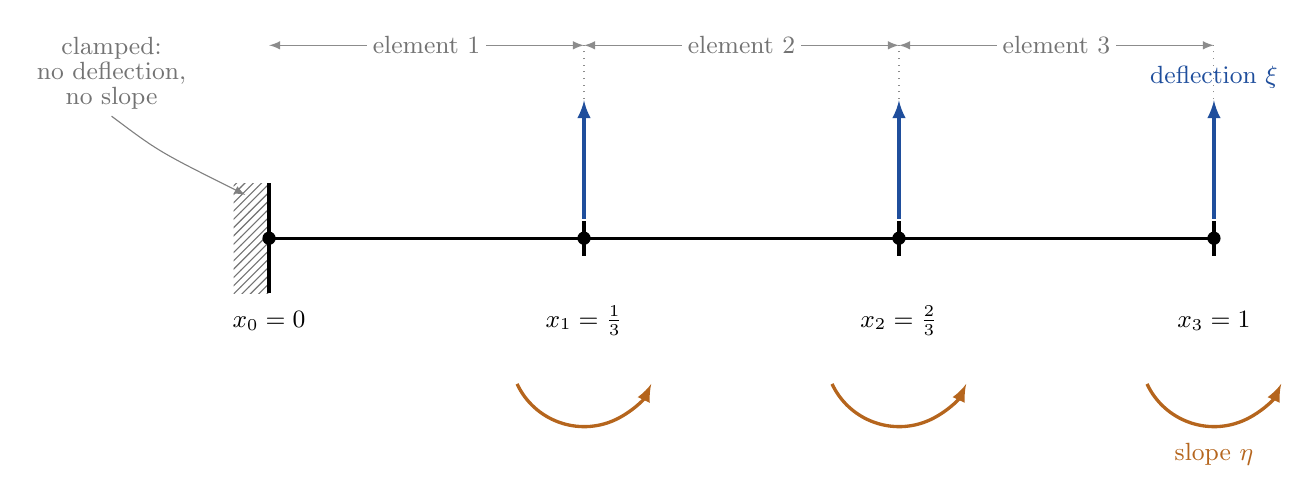
\begin{tikzpicture}[>=latex]
  % --- wall ---
  \fill[pattern=north east lines,pattern color=black!55] (-0.45,-0.7) rectangle (0,0.7);
  \draw[very thick] (0,-0.7) -- (0,0.7);
  % --- beam ---
  \draw[very thick] (0,0) -- (12,0);
  % --- element spans (above everything) ---
  \foreach \a/\b/\lab in {0/4/{element 1},4/8/{element 2},8/12/{element 3}}{
     \draw[<->,black!45] (\a,2.45) -- (\b,2.45);
     \node[fill=white,inner sep=2pt,font=\small,text=black!55] at ({(\a+\b)/2},2.45) {\lab};}
  \draw[black!45,dotted] (4,0.25) -- (4,2.45);
  \draw[black!45,dotted] (8,0.25) -- (8,2.45);
  \draw[black!45,dotted] (12,0.25) -- (12,2.45);
  % --- nodes ---
  \foreach \x/\lab in {0/{x_0=0},4/{x_1=\tfrac13},8/{x_2=\tfrac23},12/{x_3=1}}{
     \draw[very thick] (\x,-0.22) -- (\x,0.22);
     \fill (\x,0) circle (2.4pt);}
  \node[font=\small] at (0,-1.05)  {$x_0=0$};
  \node[font=\small] at (4,-1.05)  {$x_1=\tfrac13$};
  \node[font=\small] at (8,-1.05)  {$x_2=\tfrac23$};
  \node[font=\small] at (12,-1.05) {$x_3=1$};
  % --- deflection dofs (up arrows) ---
  \foreach \x in {4,8,12}{\draw[->,very thick,DeflC] (\x,0.25) -- (\x,1.75);}
  \node[font=\small,text=DeflC,align=center] at (12,2.05) {deflection $\xi$};
  % --- slope dofs (curved arrows, clear of the labels) ---
  \foreach \x in {4,8,12}{
     \draw[->,very thick,SlopC] ({\x-0.85},-1.85) arc[start angle=205,end angle=335,radius=0.94];}
  \node[font=\small,text=SlopC,align=center] at (12,-2.75) {slope $\eta$};
  % --- clamped annotation ---
  \draw[->,black!50] (-2.0,1.55) .. controls (-1.4,1.1) .. (-0.3,0.55);
  \node[font=\small,align=center,text=black!55] at (-2.0,2.1)
        {clamped:\\[-2pt]no deflection,\\[-2pt]no slope};
\end{tikzpicture}
\end{center}

\textbf{Which node keeps its unknowns.}
\begin{center}\small
\renewcommand{\arraystretch}{1.25}
\begin{tabular}{@{}llll@{}}
\toprule
node & position & what the problem says & unknowns there\\
\midrule
$x_{0}$ & $0$ & clamped: $u(0)=0$ and $u'(0)=0$ & \textbf{none} --- both are known to be $0$\\
$x_{1}$ & $1/3$ & nothing & deflection, slope\\
$x_{2}$ & $2/3$ & nothing & deflection, slope\\
$x_{3}$ & $1$ & free end: no deflection or slope is prescribed & deflection, slope\\
\bottomrule
\end{tabular}
\end{center}

So there are \textbf{six unknown numbers}.  Everything below is a list of six
things.

\section*{1. The six unknowns}

Two names, because there are two \emph{kinds} of unknown:

\[
  \underbrace{\xi_{1},\ \xi_{2},\ \xi_{3}}_{\textstyle\text{\textbf{deflections} (how far the beam moved)}}
  \qquad\qquad
  \underbrace{\eta_{1},\ \eta_{2},\ \eta_{3}}_{\textstyle\text{\textbf{slopes} (how much it tilted)}}
\]

\begin{center}\small
\renewcommand{\arraystretch}{1.25}
\begin{tabular}{@{}lll@{}}
\toprule
symbol & read it as & it equals\\
\midrule
$\xi_{1}$  & ``deflection at node 1'' & $U(1/3)$\\
$\xi_{2}$  & ``deflection at node 2'' & $U(2/3)$\\
$\xi_{3}$  & ``deflection at node 3'' & $U(1)$\\
$\eta_{1}$ & ``slope at node 1''      & $U'(1/3)$\\
$\eta_{2}$ & ``slope at node 2''      & $U'(2/3)$\\
$\eta_{3}$ & ``slope at node 3''      & $U'(1)$\\
\bottomrule
\end{tabular}
\end{center}

The subscript is \textbf{the node number and nothing else}.  $\xi$ and $\eta$
are just two different letters so you can tell a deflection from a slope.

\section*{2. The six basis functions}

Each unknown needs one function to carry it, so there are six of those too
--- $\phi^{(\text{kind})}_{\text{node}}$, as set out on page 1.  The complete
list is
\[
  \underbrace{\phi^{(1)}_{1},\ \phi^{(1)}_{2},\ \phi^{(1)}_{3}}_{\text{\textcolor{DeflC}{deflection shapes}}}
  \qquad\qquad
  \underbrace{\phi^{(2)}_{1},\ \phi^{(2)}_{2},\ \phi^{(2)}_{3}}_{\text{\textcolor{SlopC}{slope shapes}}}
\]

and here they are, drawn on this exact mesh:

\begin{center}
  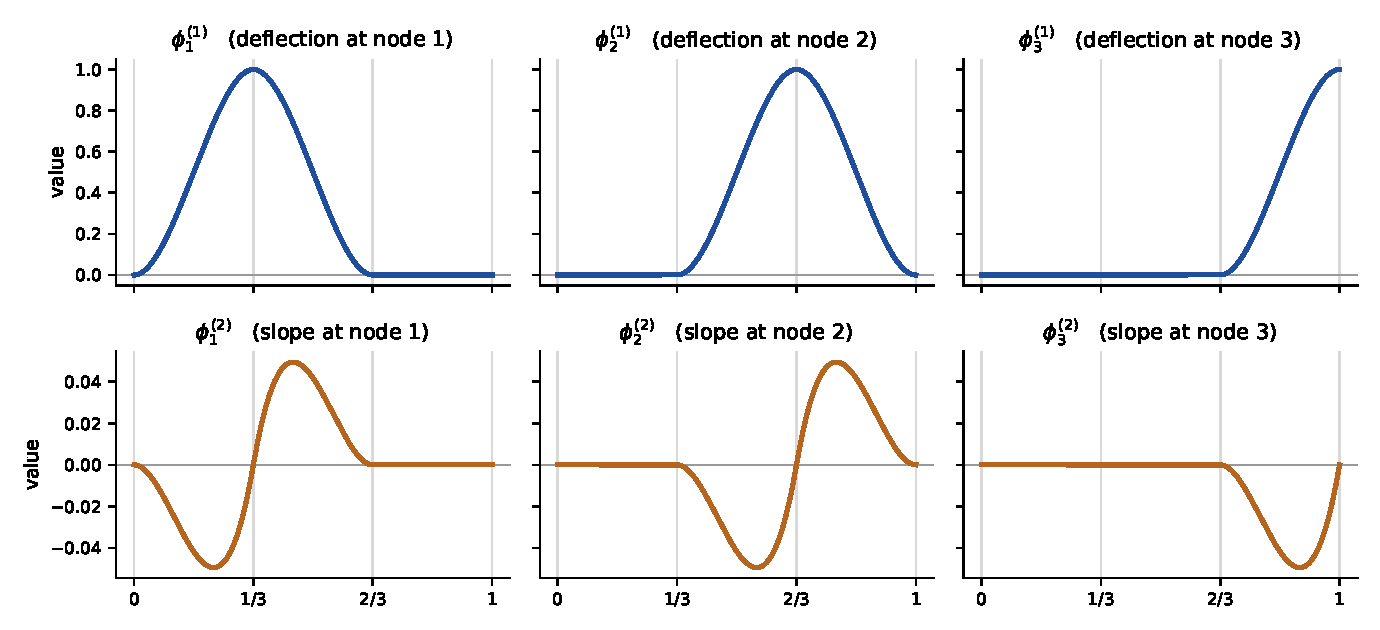
\includegraphics[width=\linewidth]{three_elem_basis.pdf}
\end{center}

Read the pictures:
\begin{itemize}\itemsep2pt
\item $\phi^{(1)}_{2}$ (top middle) is a bump of height 1 at $x=2/3$, with a
      \emph{flat top}, dying at $x=1/3$ and $x=1$.  It moves node 2 up by one
      unit and does nothing else.
\item $\phi^{(2)}_{2}$ (bottom middle) passes through \emph{zero} at $x=2/3$ but
      crosses with slope 1.  It tilts node 2 without moving it.
\item $\phi^{(1)}_{3}$ and $\phi^{(2)}_{3}$ (right column) are \textbf{half} the
      width of the others: node 3 is the free tip, so it has an element on its
      left only.
\end{itemize}

\section*{3. The approximate solution, written out}

No summation sign --- there are only six terms:
\[
  \boxed{\;
  U(x)=\xi_{1}\phi^{(1)}_{1}(x)+\xi_{2}\phi^{(1)}_{2}(x)+\xi_{3}\phi^{(1)}_{3}(x)
       +\eta_{1}\phi^{(2)}_{1}(x)+\eta_{2}\phi^{(2)}_{2}(x)+\eta_{3}\phi^{(2)}_{3}(x)\;}
\]

\section*{4. Why the shapes are built that way: the table is an identity matrix}

Take each of the six functions and make all six measurements on it --- its value
at the three nodes and its slope at the three nodes.  (Computed, not asserted.)

\begin{center}\small
\renewcommand{\arraystretch}{1.3}
\begin{tabular}{@{}l|ccc|ccc@{}}
\toprule
 & value at $\tfrac13$ & value at $\tfrac23$ & value at $1$
 & slope at $\tfrac13$ & slope at $\tfrac23$ & slope at $1$\\
\midrule
$\phi^{(1)}_{1}$ & \textbf{1} & 0 & 0 & 0 & 0 & 0\\
$\phi^{(1)}_{2}$ & 0 & \textbf{1} & 0 & 0 & 0 & 0\\
$\phi^{(1)}_{3}$ & 0 & 0 & \textbf{1} & 0 & 0 & 0\\
\midrule
$\phi^{(2)}_{1}$ & 0 & 0 & 0 & \textbf{1} & 0 & 0\\
$\phi^{(2)}_{2}$ & 0 & 0 & 0 & 0 & \textbf{1} & 0\\
$\phi^{(2)}_{3}$ & 0 & 0 & 0 & 0 & 0 & \textbf{1}\\
\bottomrule
\end{tabular}
\end{center}

\textbf{It is the $6\times6$ identity matrix.}  That is the whole design of the
basis, and it is the only reason the unknowns mean anything.  Put $x=2/3$ into
$U$ and read down the ``value at $2/3$'' column: five of the six numbers are
zero, one is 1, so
\[
  U(2/3)=\xi_{1}\cdot0+\xi_{2}\cdot\mathbf{1}+\xi_{3}\cdot0
        +\eta_{1}\cdot0+\eta_{2}\cdot0+\eta_{3}\cdot0=\xi_{2}.
\]
Differentiate and read down the ``slope at $2/3$'' column the same way:
$U'(2/3)=\eta_{2}$.

\medskip
If the table were \emph{not} the identity --- say $\phi^{(2)}_{2}$ had value
$0.3$ at $x=2/3$ instead of $0$ --- you would get
$U(2/3)=\xi_{2}+0.3\,\eta_{2}$, and $\xi_{2}$ would no longer be ``the
deflection at node 2''.  The zeros are what keep the two kinds of unknown from
contaminating each other.

\section*{5. The matrix}

Six unknowns means a $6\times6$ system.  Order them deflections-first:
$(\xi_{1},\xi_{2},\xi_{3},\eta_{1},\eta_{2},\eta_{3})$.  With $h=1/3$ the three
blocks are numbers, not symbols:

\[
  \boldsymbol{A}=\begin{bmatrix}648&-324&0\\-324&648&-324\\0&-324&\boxed{324}\end{bmatrix},\quad
  \boldsymbol{B}=\begin{bmatrix}24&6&0\\6&24&6\\0&6&\boxed{12}\end{bmatrix},\quad
  \boldsymbol{C}=\begin{bmatrix}0&54&0\\-54&0&54\\0&-54&\boxed{-54}\end{bmatrix}
\]
\[
  \begin{bmatrix}\boldsymbol{A}&\boldsymbol{C}\\[2pt]\boldsymbol{C}^{T}&\boldsymbol{B}\end{bmatrix}
  \begin{bmatrix}\xi_{1}\\\xi_{2}\\\xi_{3}\\\eta_{1}\\\eta_{2}\\\eta_{3}\end{bmatrix}
  =\begin{bmatrix}b^{(1)}_{1}\\b^{(1)}_{2}\\b^{(1)}_{3}\\b^{(2)}_{1}\\b^{(2)}_{2}\\b^{(2)}_{3}\end{bmatrix},
  \qquad
  \boldsymbol{A}_{\,\text{entry}}=\int_{0}^{1}\bigl(\phi^{(1)}\bigr)''\bigl(\phi^{(1)}\bigr)''\dx,\ \text{etc.}
\]

The \boxed{\text{boxed}} corner entries are the free tip.  Node 3 has only one
element attached instead of two, so it collects half of what an interior node
collects: $324$ instead of $648$, $12$ instead of $24$, and $-54$ instead of
$0$.

\section*{6. Worked numbers: uniform load $f=1$}

Solving the $6\times6$ system with $f\equiv1$ gives

\begin{center}\small
\renewcommand{\arraystretch}{1.3}
\begin{tabular}{@{}llllll@{}}
\toprule
node & $x$ & FEM deflection & exact $u(x)$ & FEM slope & exact $u'(x)$\\
\midrule
1 & $1/3$ & $\xi_{1}=0.022119$ & $0.022119$ & $\eta_{1}=0.117284$ & $0.117284$\\
2 & $2/3$ & $\xi_{2}=0.069959$ & $0.069959$ & $\eta_{2}=0.160494$ & $0.160494$\\
3 & $1$   & $\xi_{3}=0.125000$ & $0.125000$ & $\eta_{3}=0.166667$ & $0.166667$\\
\bottomrule
\end{tabular}
\end{center}

with $u(x)=\dfrac{x^{2}(x^{2}-4x+6)}{24}$ the exact solution.  The nodal values
agree to $3\times10^{-15}$ --- with only three elements.

\medskip
And the tip numbers are the two formulas from any statics table, with
$w=1$, $L=1$, $EI=1$:
\[
  \xi_{3}=\frac18=\frac{wL^{4}}{8EI}\quad\text{(tip deflection)},
  \qquad
  \eta_{3}=\frac16=\frac{wL^{3}}{6EI}\quad\text{(tip rotation)} .
\]

\vfill
{\footnotesize\color{black!55}All numbers in Sections 4, 5 and 6 were computed,
not quoted: the nodal table by evaluating the six functions, the blocks by Gauss
quadrature against the element integrals, and Section 6 by solving the
$6\times6$ system.  Script: \texttt{three\_elem\_basis.py}.}

\end{document}
